% use pdfpc to present
\documentclass[]{beamer}

\usepackage{color}
\usepackage{pgfpages}
\usepackage{url}
\usepackage{hyperref}

\setbeameroption{show notes on second screen=right}

%TODO: Add Images

%document specific info
\title{Physical Security}
\subtitle{or ``Why is that man in my server room''}
\author{Stephen ``ToxicSauce'' Walker-Weinshenker}
\institute{
  \inst{}
  Department of Computer Science\\
  Colorado State University
  \and
  \inst{}
  Department of Electrical and Computer Engineering\\
  Colorado State University
}
\date{\today}
\subject{subject}

%beamer template
\definecolor{HDred}{RGB}{171,31,36}
\setbeamercolor{background canvas}{bg=gray}
\setbeamercolor{title}{fg=HDred}
\setbeamercolor{frametitle}{fg=HDred}
\setbeamercolor{logo}{bg=gray}

\logo{
\includegraphics[height=1.5cm]{logo.png}}

\useoutertheme[hideallsubsections]{sidebar}


\begin{document}
\frame{\titlepage}

% \begin{frame}
% \frametitle{Table of Contents}
% \tableofcontents%[current section]
% \end{frame}

\begin{frame}
  \frametitle{What is Physical Security}
\begin{itemize}
  \item Controlling physical access to something
  \item Normally used in the context of a building or room
\end{itemize}
\begin{alertblock}{Note:}
  Any type of Security is a balance between security, convience of access and aesthetics.
\end{alertblock}
\note[item]{there is no perfect security}
\end{frame}

\begin{frame}
  \frametitle{Primary Elements of Physical Security}
\begin{itemize}
  \item Physical Structure of Building and Site
  \begin{itemize}
    \item Doors
    \item Windows
    \item Walls
    \item Roofs
    \item Floors
    \item Perimeter of Property
  \end{itemize}
\end{itemize}

\end{frame}



\begin{frame}
  \frametitle{Primary Elements of Physical Security}
\begin{itemize}
  \item Secure Elements of Building
  \begin{itemize}
    \item Locks and Keys
    \item Other Access Control
    \item Man Traps
    \item Vehicle Gates
  \end{itemize}
\end{itemize}

\end{frame}

\begin{frame}
  \frametitle{Human Factors}
\begin{itemize}
  \item Security Guards
  \item Other Employees

\end{itemize}
\end{frame}

\begin{frame}
  \frametitle{Security Guards}
  \begin{columns}[c]
    \column{0.5\textwidth}
    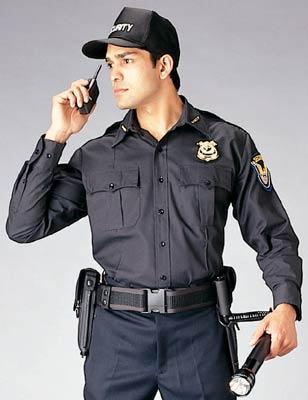
\includegraphics[width=.8\textwidth]{Security-Guard}
    \column{0.5\textwidth}
    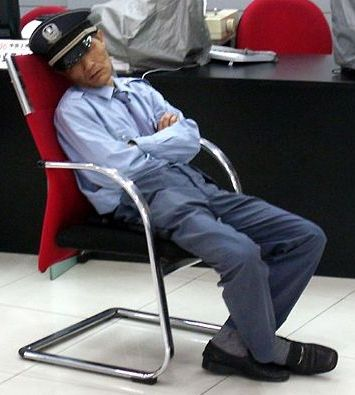
\includegraphics[width=0.8\textwidth]{Security-Guard-Sleeping}
  \end{columns}
\note[item]{is there a way around the guards}
\note[item]{how attentive are they}
\note[item]{are they distracted}
\note[item]{can they be distracted}

\end{frame}



\begin{frame}
  \frametitle{Other Employees}
  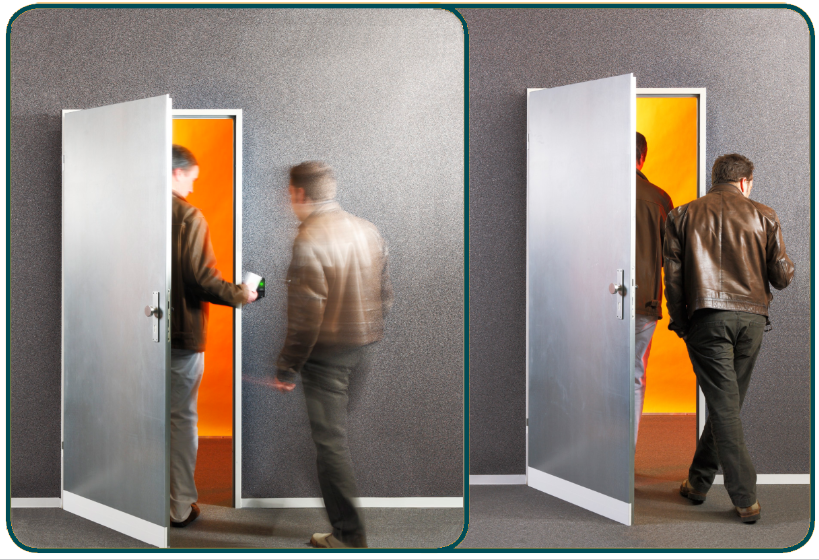
\includegraphics[width=.9\textwidth]{tailgating}
  \note[item]{tailgating}
  \note[item]{social engineering}
  \note[item]{bribery}
\end{frame}

\begin{frame}
  \frametitle{Doors}
  \begin{columns}[c]
    \column{0.5\textwidth}
  \begin{itemize}
    \item frame gap
    \item REX sensor
    \item lock --- fail safe or deadly
    \item hinges
    \item door fit
  \end{itemize}
  \column{0.5\textwidth}
  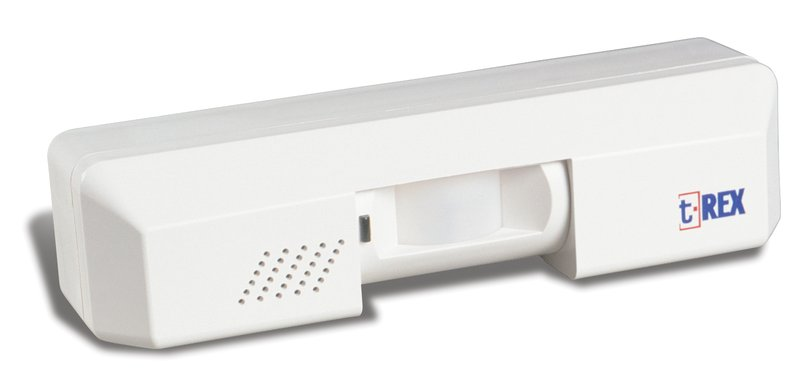
\includegraphics[width=0.9\textwidth]{T-REX}
\end{columns}
\note[item]{\url{https://www.youtube.com/watch?v=SDl4AO4ancI}}
\end{frame}

\begin{frame}
  \frametitle{Windows}
  \begin{columns}[c]<1->
    \column{0.5\textwidth}
    \begin{block}{Fooled you}
      No not this windows
    \end{block}
    \column{0.5\textwidth}
    
\includegraphics[width=0.9\textwidth]{Windows_10_Hero}
  \end{columns}
  \vspace{1mm}
  \begin{columns}[c]<2-2>
    \column{0.5\textwidth}
    These windows
    \column{0.5\textwidth}
    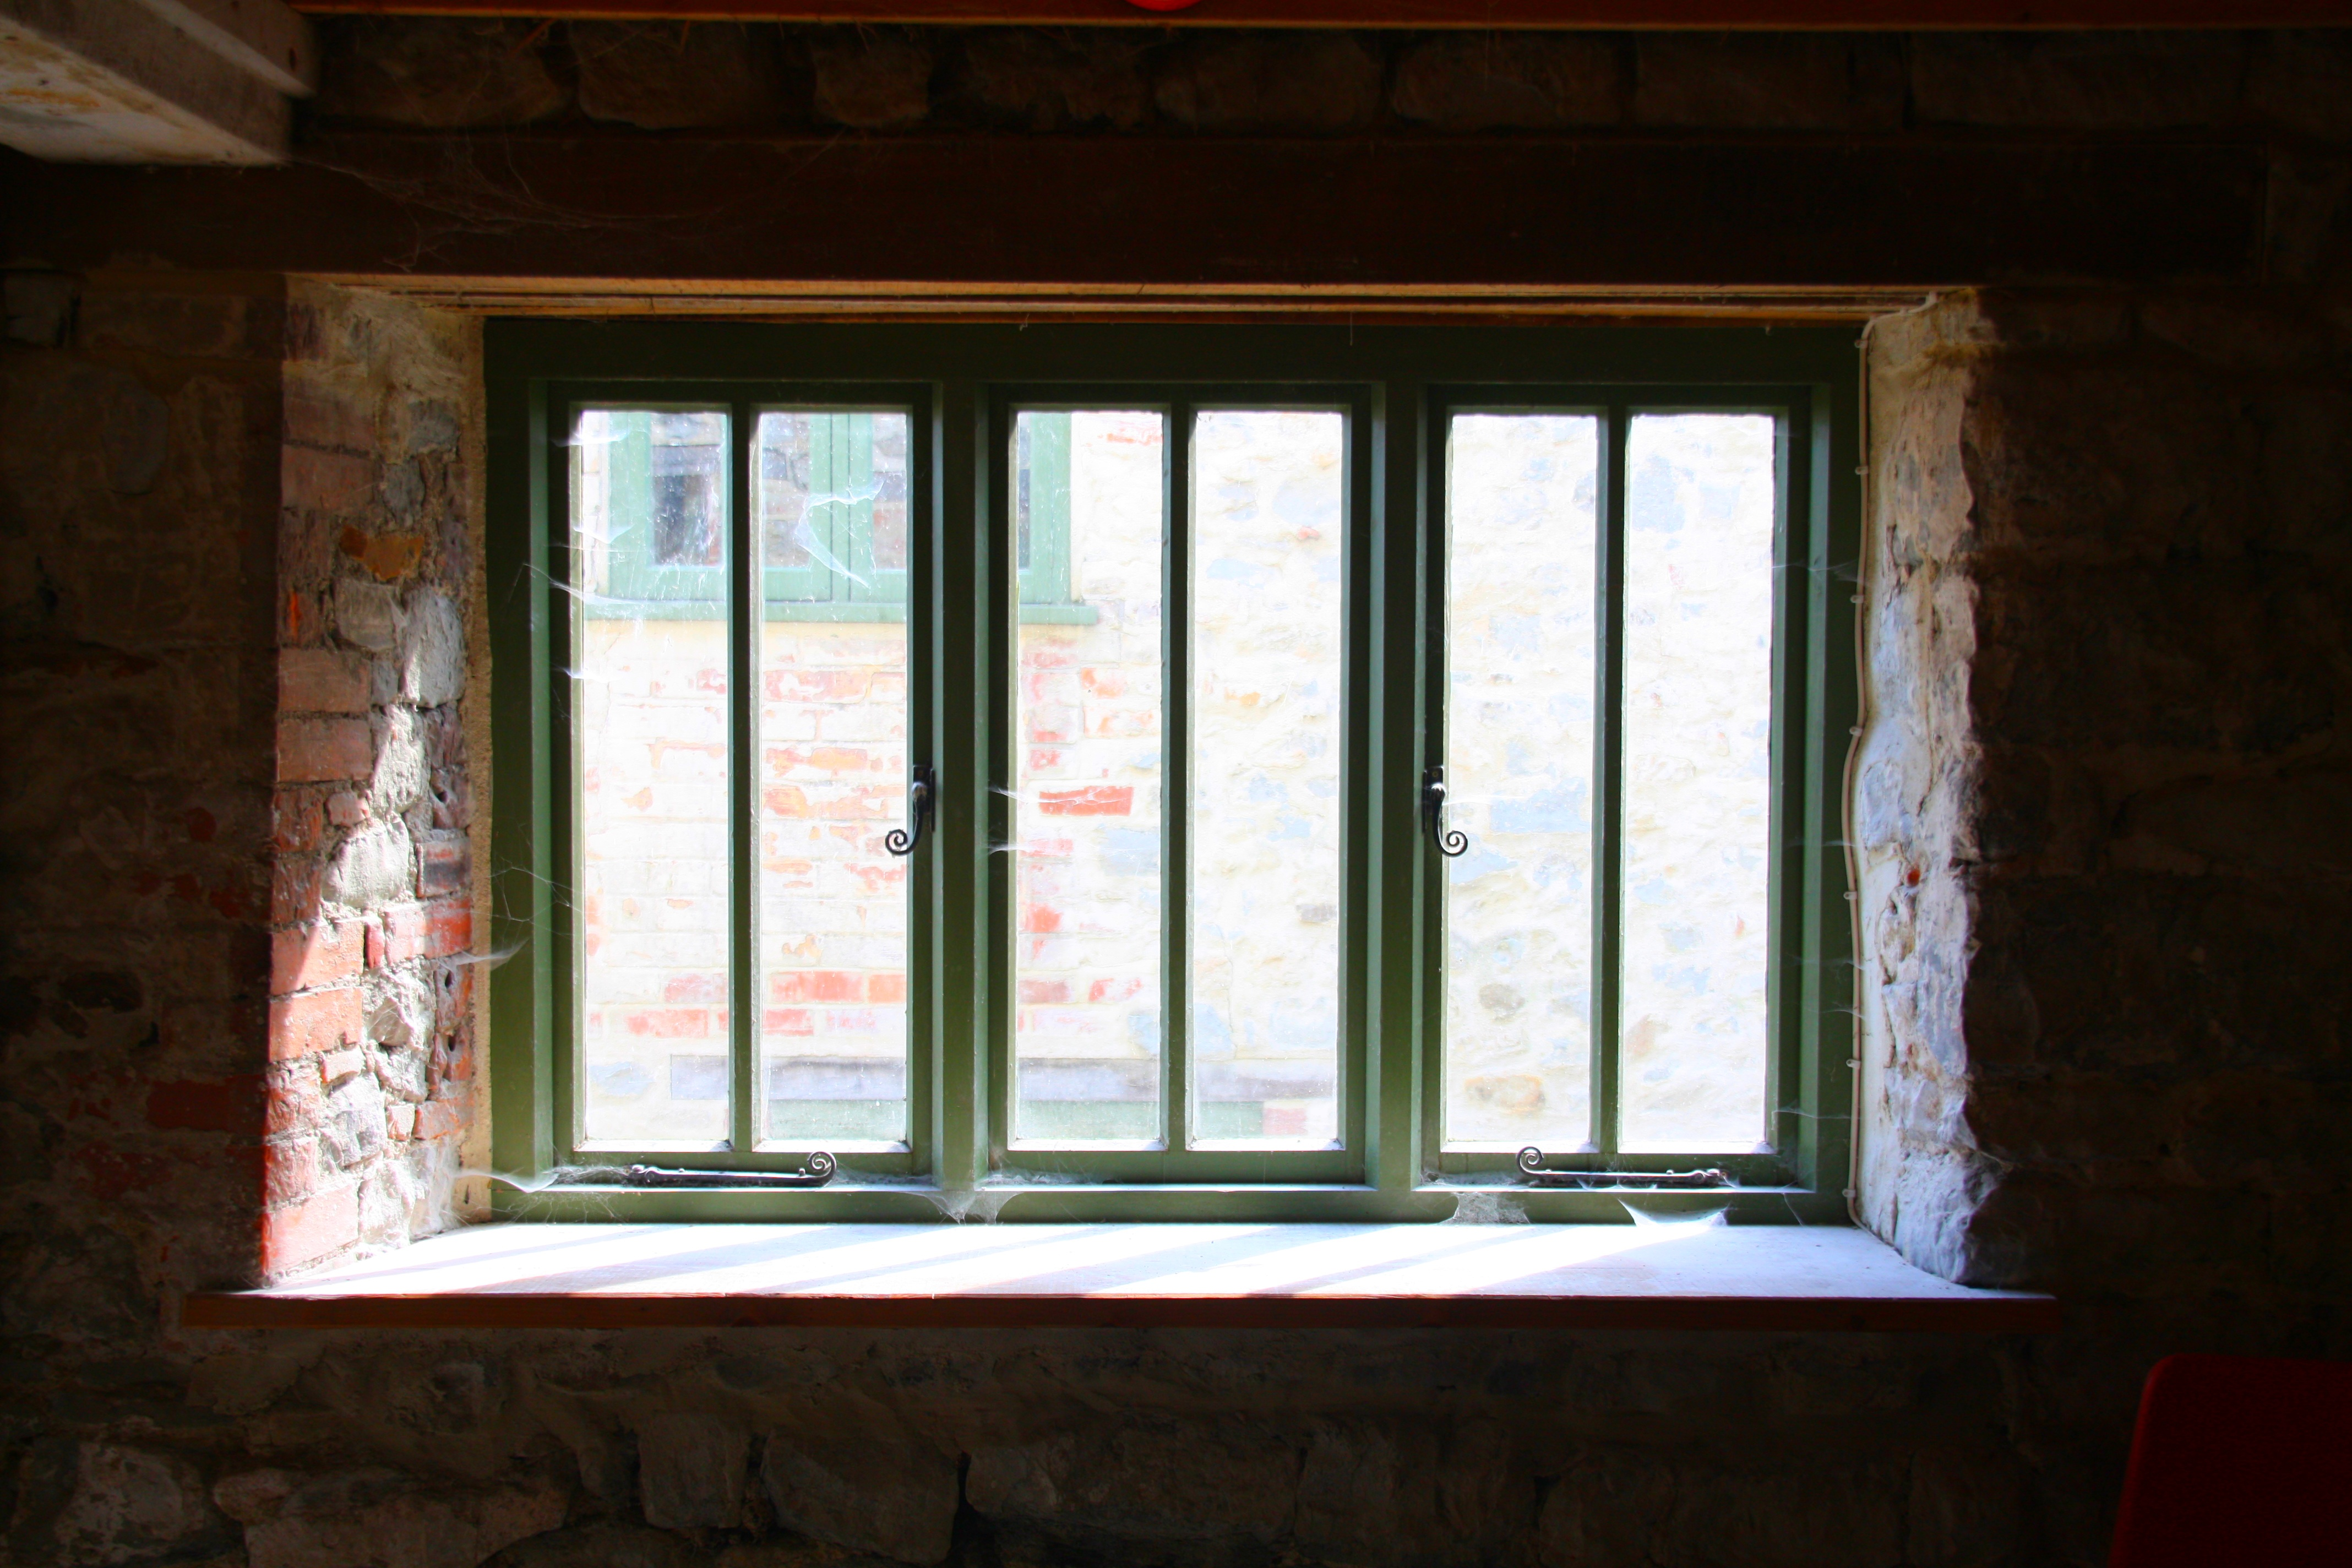
\includegraphics[width=0.9\textwidth]{Window}
  \end{columns}
  \note[item]{blinds}
  \note[item]{potentially bars, don't want to appear that you are protecting something}
  \note[item]{security film/glass/fire rated glass}
  \note[item]{windows higher up on wall, without ledges}
\end{frame}

\begin{frame}
  \frametitle{Walls/Roofs/Floors}
  \begin{itemize}
    \item solid construction. Tisue paper != secure
    \item for roofs, steep slopes are harder to stand on
    \item skylights instead of windows except in case of helicopters
    \item think about mechanical equipment on roof as another access point / potential attack surface
  \end{itemize}
\end{frame}

\begin{frame}
  \frametitle{Perimeter of Property}
  \begin{columns}[c]
    \column{0.5\textwidth}
    \begin{itemize}
      \item vehicle gates
      \item natural vegetation
      \item open areas between buildings and surroundings
    \end{itemize}
    \column{0.5\textwidth}
    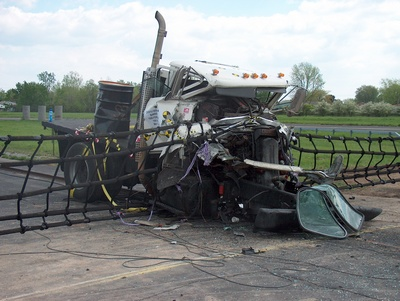
\includegraphics[width=0.9\textwidth]{vehicle-impact2}
    \vspace{2mm}
    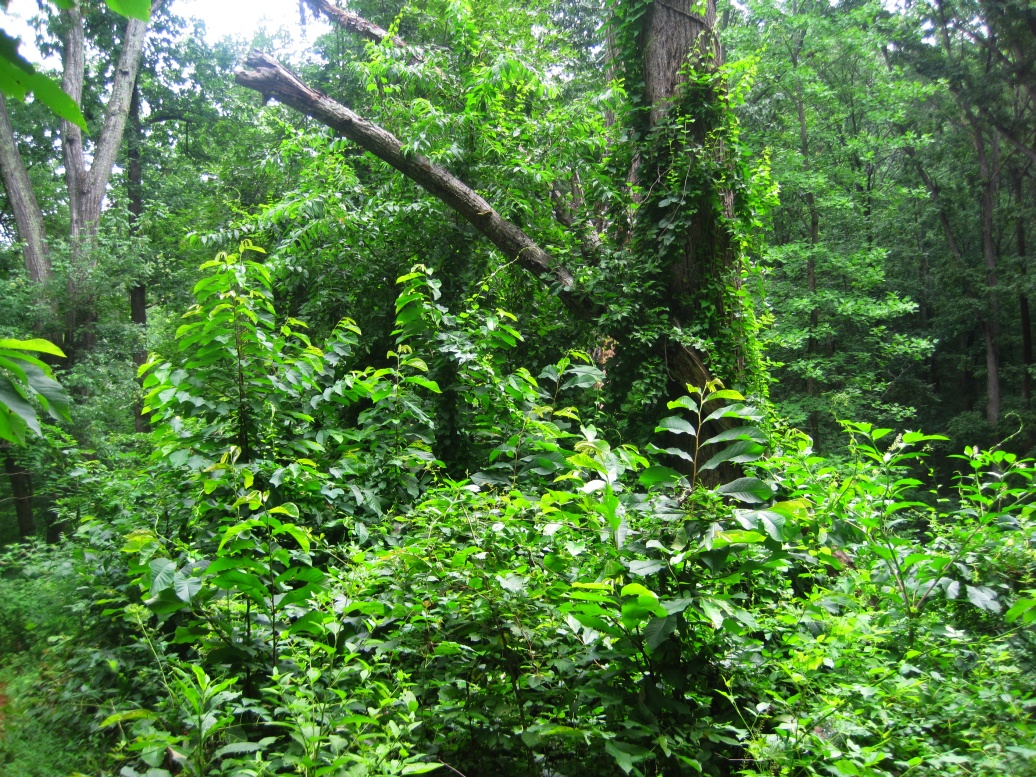
\includegraphics[width=0.9\textwidth]{vegetation}
  \end{columns}
\end{frame}

\begin{frame}
  \frametitle{Locks and Keys}
  \begin{columns}[c]
    \column{0.5\textwidth}
    \begin{itemize}
      \item most locks are shit
      \item almost all padlocks are shit
      \item good locks are not infaliable
      \item master keys/recorable locks
      \item keyboxen --- knox boxen
    \end{itemize}
    \column{0.5\textwidty}
    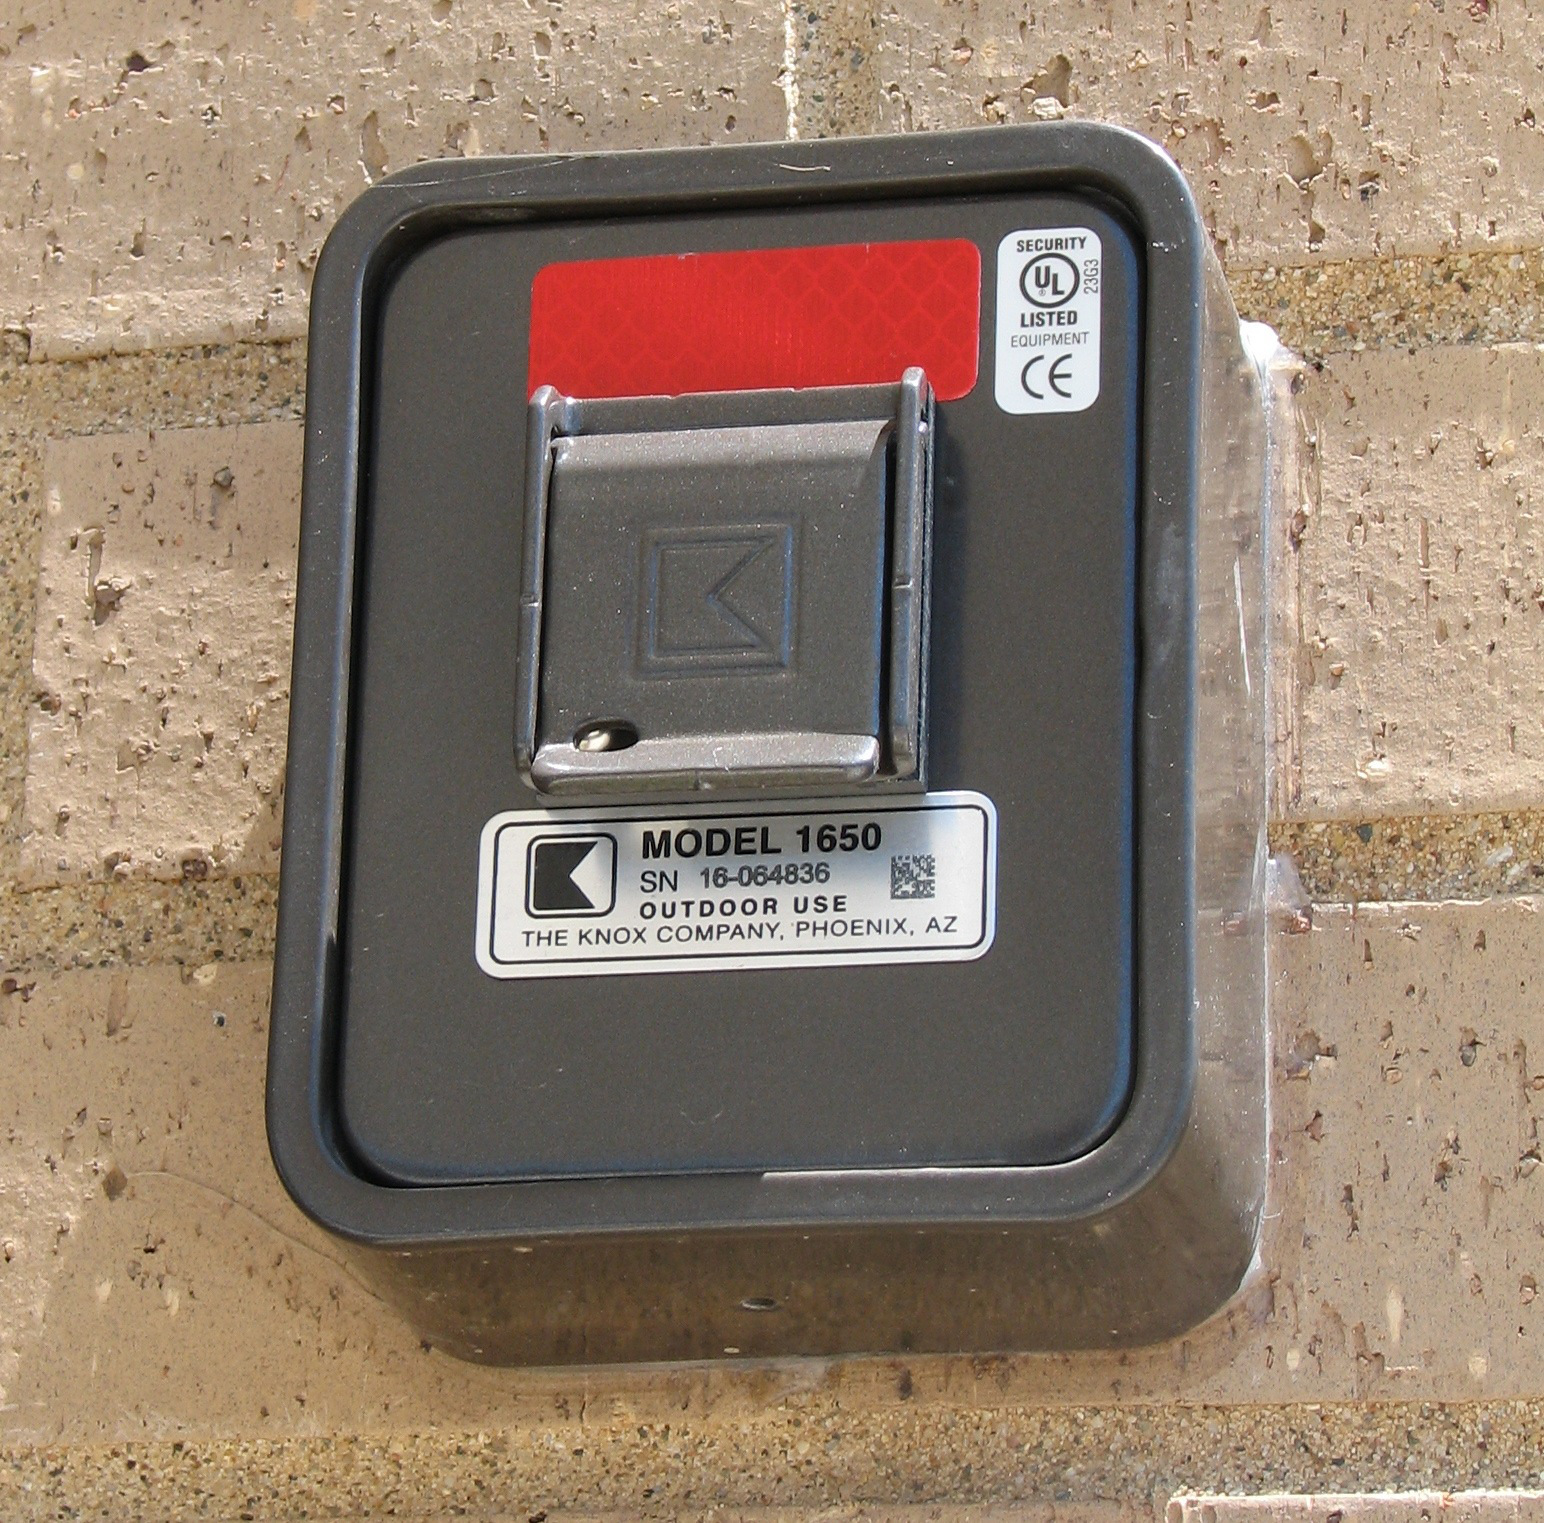
\includegraphics[width=0.9\textwidth]{Knox-Box}
    
\includegraphics[width=0.9\textwidth]{masterlock}
    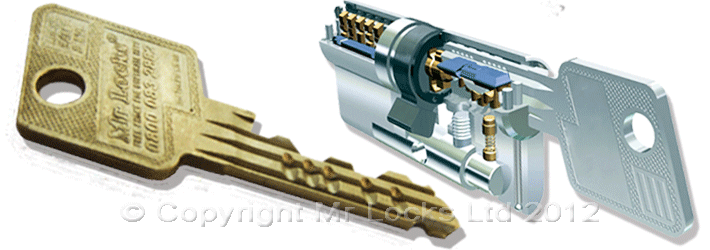
\includegraphics[width=0.9\textwidth]{high-sec-lock}
  \end{columns}

\end{frame}

\begin{frame}
  \frametitle{Other Access Control/CCTV}
  \begin{columns}
    \column{0.5\textwidth}
    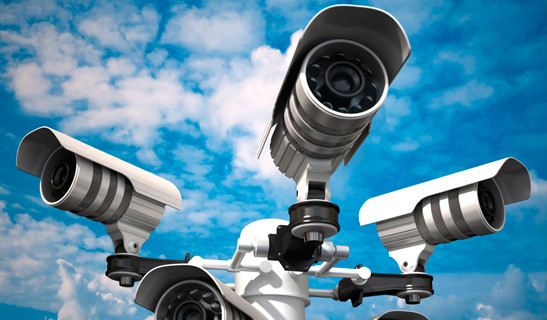
\includegraphics[width=0.9\textwidth]{cctv}
    \column{0.5\textwidth}
    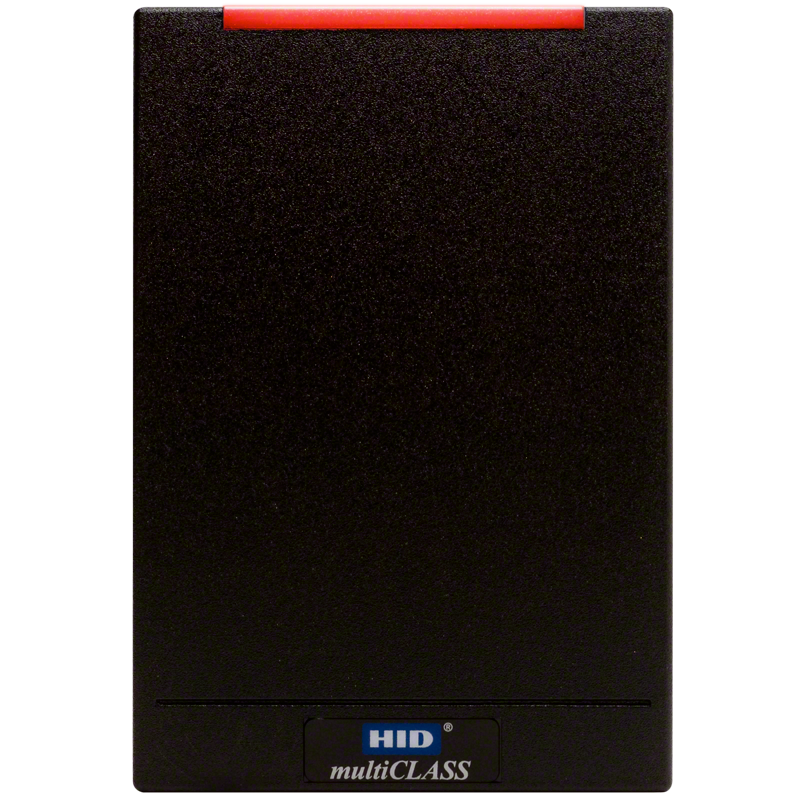
\includegraphics[width=0.9\textwidth]{hid-reader}
  \end{columns}
\end{frame}

\begin{frame}
  \frametitle{Man Traps}
  \begin{columns}
    \column{0.5\textwidth}
    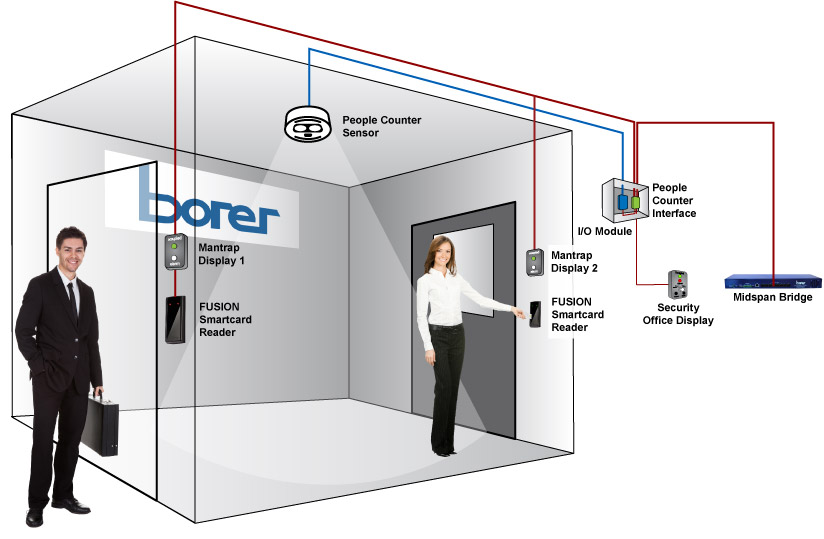
\includegraphics[width=0.9\textwidth]{access-control-mantrap}
    \column{0.5\textwidth}
    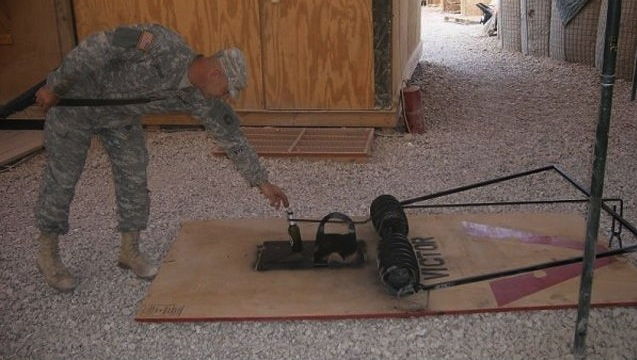
\includegraphics[width=0.9\textwidth]{Man-Trap-1}
    \includegraphics[width=0.9\textwidth]{Man-Trap-2}
  \end{columns}
\end{frame}

\begin{frame}
  \frametitle{References}
  \begin{itemize}
    \item \url{http://www.securityguardpedia.com/wp-content/uploads/2015/02/Security-Guard-East-Region.jpg}
    \item \url{http://kudos-security.com/wp-content/uploads/2015/06/TAILGATING.png}
    \item \url{http://cms.dsc.com/media/products/lthumbs/i_T-REX.jpg}
    \item \url{https://www.youtube.com/watch?v=4YYvBLAF4T8}
    \item \url{https://upload.wikimedia.org/wikipedia/commons/8/8c/Bank-Security-Guard-Sleeping-Cropped.jpeg}
    \item \url{http://blogs-images.forbes.com/patrickmoorhead/files/2015/08/Windows_10_Hero.png}
    \item \url{https://upload.wikimedia.org/wikipedia/commons/5/54/WaterMill_Window_LymeRegis.jpg}
    \item \url{http://www.nationwidestructures.com/barrier/vehicle-impact2.jpg}
    \item \url{https://yearinthewoods.files.wordpress.com/2013/07/img_1314.jpg}
    \item \url{http://danvillefire.org/dfdwp/wp-content/uploads/2013/03/Knox-Box.jpg}
    \item \url{https://www.hidglobal.com/sites/default/files/rp40_blk_6125_6123_6124_3.png}
    \item \url{http://cdn.small.masterlock.com/masterlock/resources/img/home-content-boxes/product-selector-personal.png}
    \item \url{http://www.locksmithcowbridge.co.uk/assets/img/cowbridge-locksmith-high-security-registered-profile-locks.png}
    \item \url{http://saysthesinglegirl.com/wp-content/uploads/2012/01/Man-Trap.jpg}
    \item \url{http://1funny.com/wp-content/uploads/2011/03/man-trap.jpg}
    \item \url{http://www.mantrap.solutions/images/access-control-mantrap.jpg}
    \item \url{http://addontechno.com/wp-content/uploads/2015/02/eye-in-every-corner-547x320.jpg}
  \end{itemize}

\end{frame}

\end{document}
